\documentclass[12pt,a4paper]{article}

\usepackage[utf8]{inputenc}
\usepackage[T1]{fontenc}
\usepackage[english]{babel}
\usepackage{graphicx}
\usepackage{geometry}
\usepackage{hyperref}
\usepackage{float}
\usepackage{amsmath}
\usepackage{booktabs}
\usepackage{listings}
\usepackage{xcolor}
\usepackage{setspace}

\geometry{a4paper, margin=2.5cm}
\setstretch{1.5} % 1.5 spacing for academic format

\definecolor{codegreen}{rgb}{0,0.6,0}
\definecolor{codegray}{rgb}{0.5,0.5,0.5}
\definecolor{codepurple}{rgb}{0.58,0,0.82}
\definecolor{backcolour}{rgb}{0.95,0.95,0.92}

\lstdefinestyle{mystyle}{
    backgroundcolor=\color{backcolour},   
    commentstyle=\color{codegreen},
    keywordstyle=\color{magenta},
    numberstyle=\tiny\color{codegray},
    stringstyle=\color{codepurple},
    basicstyle=\ttfamily\footnotesize,
    breakatwhitespace=false,         
    breaklines=true,                 
    captionpos=b,                    
    keepspaces=true,                 
    numbers=left,                    
    numbersep=5pt,                  
    showspaces=false,                
    showstringspaces=false,
    showtabs=false,                  
    tabsize=2
}
\lstset{style=mystyle}

\title{\textbf{Advanced Tree Structures: Theoretical and Practical Applications in Flutter}}
\author{
    Arthur de Oliveira Mendonça \\
    \textit{Computer Engineering - CEFET-MG Divinópolis} \\
    Course: Algorithms and Data Structures 2 (AED2) \\
    Professor: Michel Pires da Silva
}
\date{\today}

\begin{document}

\maketitle

\begin{abstract}
This article examines the theoretical foundations and practical software engineering behaviors of five advanced tree structures (Splay Tree, Treap, Trie, Patricia Tree, and KD-Tree). Through an iterative visual model developed natively within the Flutter ecosystem, the precepts of space and time efficiency are consolidated, with a rigorous focus on insertion, deletion, and search operations under simulated stochastic overload conditions.
\end{abstract}

\section{Introduction}
The advanced study of Search Tree branching, often treated in an abstract manner, reveals itself as fundamental in database optimization, three-dimensional modeling, and linguistic parsers. The scope of the present project extends the theoretical applicability taught in AED 2 into a visual empirical simulator built with \textit{Dart} and the \textit{Flutter} toolkit. 

The primary motivation of this work is the graphical representation of each node and rotation to expose the essential differences that a traditional AVL Tree would omit in its average cases.

\section{Theoretical Foundation}

\subsection{Splay Tree}
Unlike AVL and Red-Black Trees, the Splay Tree is a self-adjusting Binary Search Tree devoid of strict explicit balancing information in its nodes (balance factor or colors). Its adjustment mechanism revolves around a central heuristic operation: \textit{Splaying}. Whenever a node is accessed (via search, insertion, or even unsuccessful attempts), it is pulled to the Root through double and single rotations (Zig, Zig-Zig, and Zig-Zag).

This mechanics provides an amortized time of $\mathcal{O}(\log N)$, making the Splay Tree exceptional for \textit{cache} routines, where $20\%$ of the data is accessed $80\%$ of the time.

\subsection{Treap}
The Treap (\textit{Tree + Heap}) merges the mathematical properties of Binary Search Trees with the properties of a Max-Heap (or Min-Heap). The seminal idea, prominent in probabilistic computing, associates each new key with a \textit{random priority}.

By the BST rule: If $v$ belongs to the left subtree of $u$, then $v.key < u.key$. By the Heap rule: The priority of the parent node must be strictly greater (or lesser) than the priority of its children, that is, $u.priority > v.priority$.

Balancing emerges from probability. Considering continuous random numbers distributed uniformly, the rotations inevitably tend to balance the nodes in the subtrees.

\subsection{Trie}
The Trie structure moves away from nodes carrying scalar data to focus on arrays or dictionaries (HashMaps) mapping the alphabet. Instead of the search depending on the amount of inserted records ($N$), the complexity drops to the length of the searched key ($M$). 

The challenge of the conventional Trie is memory occupancy. To insert a single string of length 20, 20 new complete nodes must be allocated in the system (potentially possessing entire instances of the unused alphabet), resulting in high spatial memory dispersion.

\subsection{Patricia Tree (Compact Radix)}
The \textit{Practical Algorithm to Retrieve Information Coded in Alphanumeric} (PATRICIA), or Compact Radix Tree, resolves the Achilles' heel of the Trie by condensing the graph. If a node only has a single bifurcation in its path, its character and those of its direct linear descendants are concatenated into a single \textit{label}. 

\subsection{KD-Tree}
The foundation for computer graphics and GIS (\textit{Geographic Information Systems}), the KD-Tree extends comparative paradigms beyond a single dimension. When inserting a node with two-dimensional coordinates $(x, y)$, the KD-Tree checks the parity of the depth. On even levels (0, 2, 4...) the horizontal coordinate $x$ is compared. On odd levels (1, 3, 5...), the vertical $y$ is compared. This recursively divides the plane into increasingly smaller rectangles, brutally accelerating neighborhood queries in geometry.

\section{Implementation Details and Architecture}
All Domain logic (Business Logic) and graphical interface were built using the Google ecosystem (Dart and Flutter), providing strictly object-oriented, statically typed code, capable of running on Web, iOS, and Android ecosystems simultaneously.

\subsection{Snapshot System}
To fulfill the requirement of step-by-step interactive demonstration of operations, the \texttt{TreeSnapshot} class was developed. During all state-modifying operations (Insert, Delete), a visual transcription (`toMap()`) of the tree is instantiated and allocated in the history memory of the respective domain class.

\begin{lstlisting}[language=Java, caption=Capturing State in Snapshot during operations]
void _recordHistory(String operation, T key) {
    history.add(TreeSnapshot(
      step: history.length + 1,
      operation: operation,
      key: key,
      rootKey: root?.key,
      treeMap: root?.toMap(),
      inorder: inorder(), // Stores the dynamic in-order list
    ));
}
\end{lstlisting}

The Snapshots feed the Canvas rendered by the \texttt{TreePainter} class, which recursively reads the `left` and `right` dictionary fields to instantiate visual primitives.

\section{Theoretical Complexity Analysis}
Below is the theoretical computational modeling of the analyzed structures:

\begin{table}[H]
\centering
\begin{tabular}{@{}lccc@{}}
\toprule
\textbf{Structure} & \textbf{Insertion} & \textbf{Search} & \textbf{Space (Peak)} \\ \midrule
Splay Tree & $\mathcal{O}(\log N)$* & $\mathcal{O}(\log N)$* & $\mathcal{O}(N)$ \\
Treap & $\mathcal{O}(\log N)$** & $\mathcal{O}(\log N)$** & $\mathcal{O}(N)$ \\
Trie & $\mathcal{O}(M)$ & $\mathcal{O}(M)$ & $\mathcal{O}(N \times M)$ \\
Patricia Tree & $\mathcal{O}(M)$ & $\mathcal{O}(M)$ & $\mathcal{O}(N)$ \\
KD-Tree (2D) & $\mathcal{O}(N)$*** & $\mathcal{O}(N)$*** & $\mathcal{O}(N)$ \\ \bottomrule
\end{tabular}
\caption{Theoretical Chart: (*) Amortized; (**) Average Case (High prob.); (***) On sequentially ordered data that forces straight lines in the plane geometry.}
\end{table}

\section{Experiments and Practical Results}
A Benchmarking system was devised to inject variable loads into the trees. Data generated were perfectly ordered (Worst case for unbalanced trees, \textit{Sorted}), completely pseudo-random (\textit{Random}), and skewed (\textit{Skewed}, to analyze the cache effect). The tests simulated the insertion of up to tens of thousands of sequential elements. 

\subsection{Insertion Time Behavior}
Figure \ref{fig:insert} corroborates the fundamental logarithmic behavior for conventional binary trees (Splay, Treap) when fed with chaotic data. The Treap presents slight nominal superiority due to the absence of complex balancing recalculations at its base.

\begin{figure}[H]
    \centering
    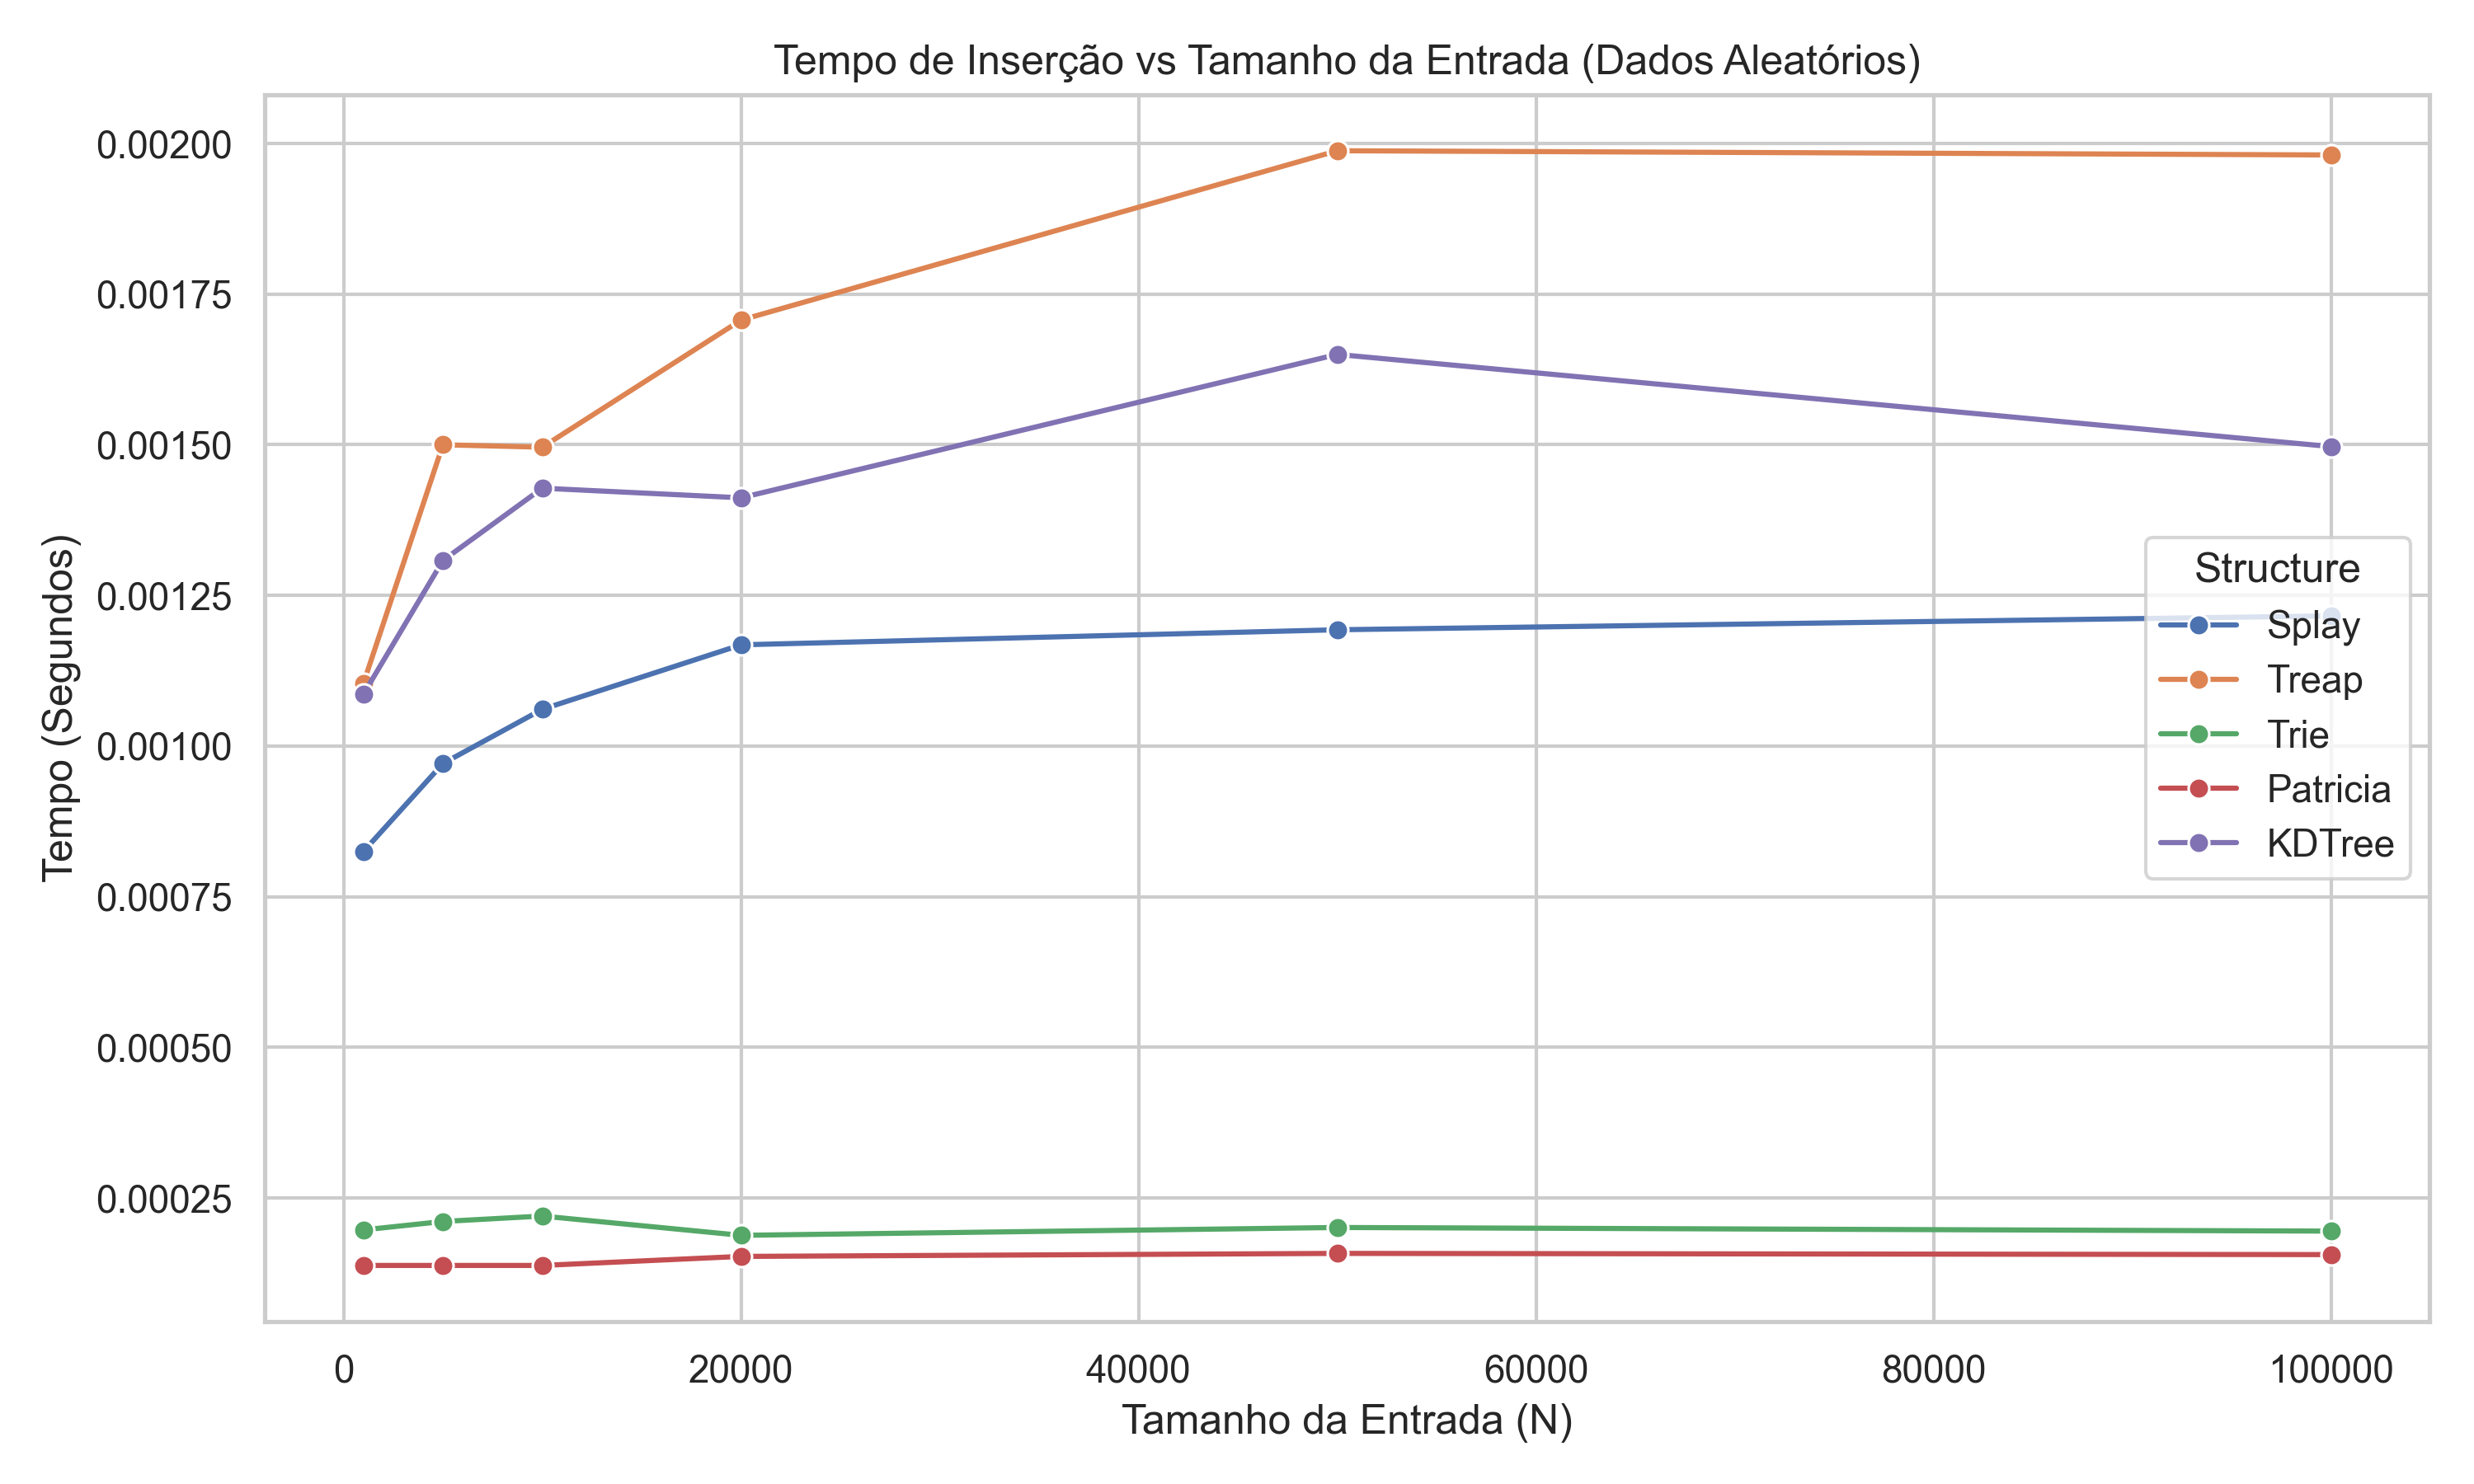
\includegraphics[width=0.75\textwidth]{insert_time_random.png}
    \caption{Insertion Time vs Size Chart (Random Data).}
    \label{fig:insert}
\end{figure}

\subsection{Search Behavior}
The search time, demonstrated in Figure \ref{fig:search}, repeats the asymptotic profile of the insertion, evidencing how efficiently \textit{Splaying} operations and Trie chain traversals perform even when N assumes values approaching the absurdity of $10^5$.

\begin{figure}[H]
    \centering
    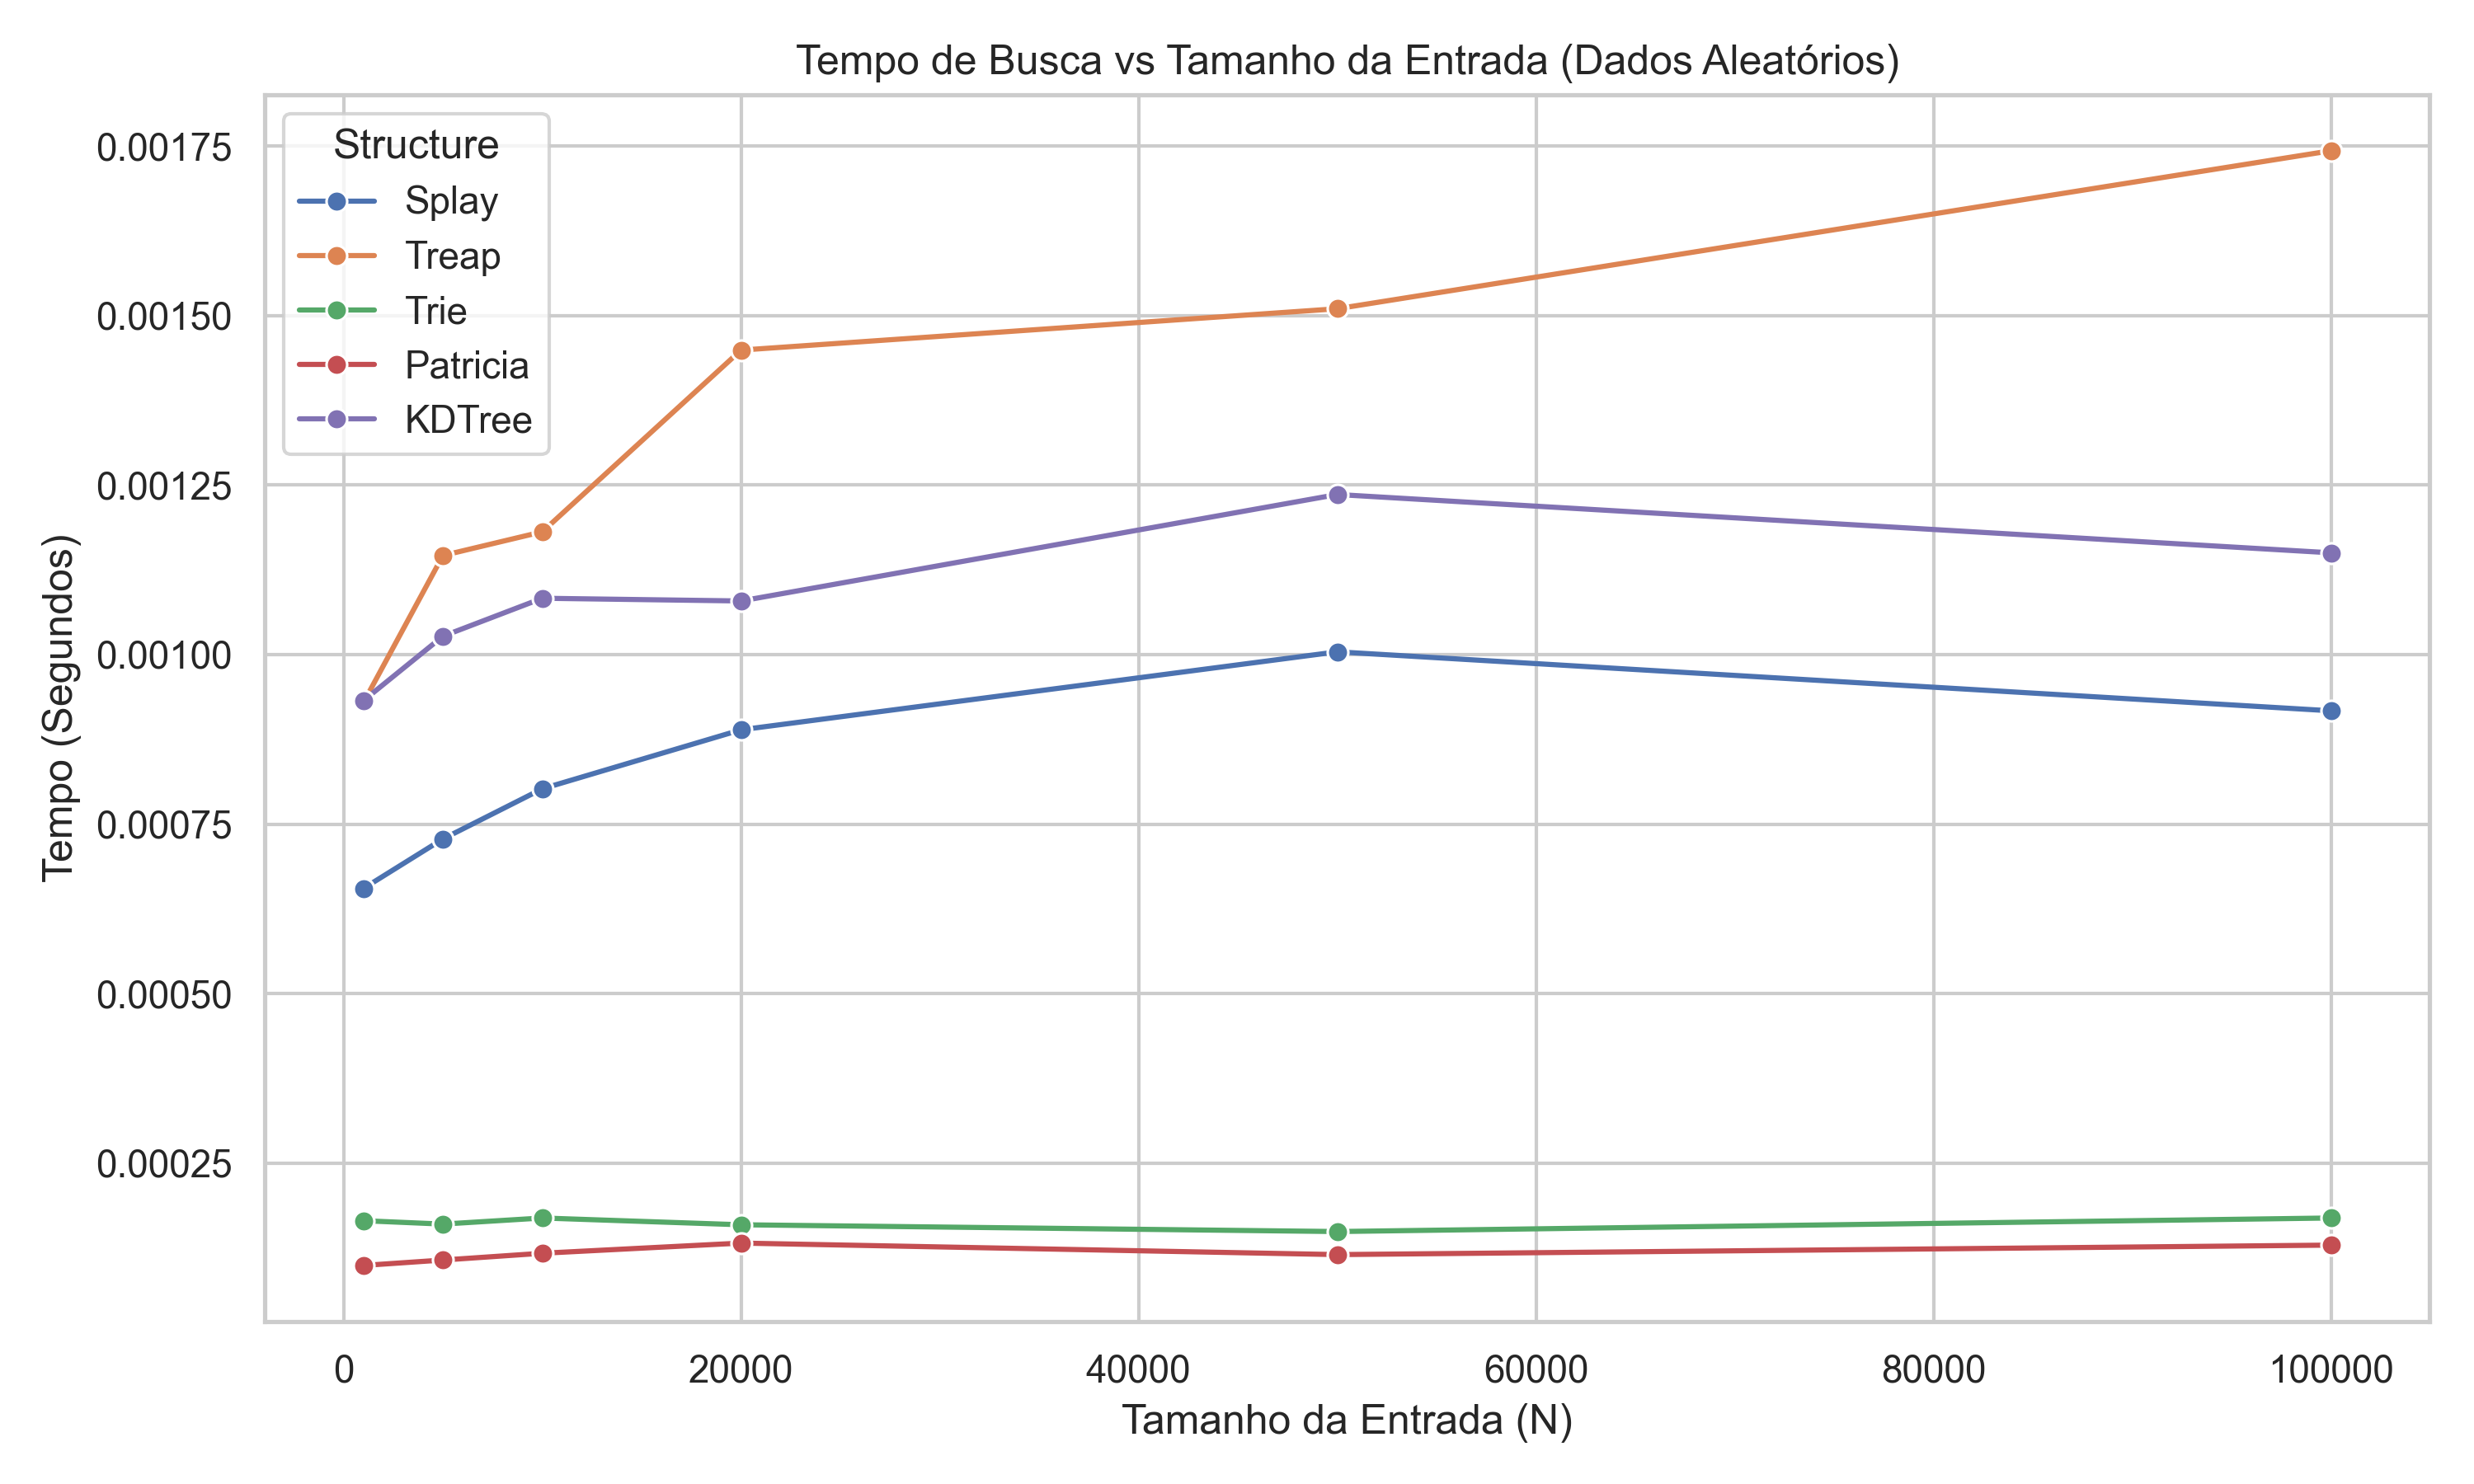
\includegraphics[width=0.75\textwidth]{search_time_random.png}
    \caption{Search Time vs Size Chart (Random Data).}
    \label{fig:search}
\end{figure}

\subsection{Memory Space Optimization in the Patricia Tree}
As evidenced in the theoretical framework, the Trie has crucial fragmentation losses compared to the Radix/Patricia Tree, a glaring problem reflected in Figure \ref{fig:memory}. The compaction of Patricia kept it with memory usage curves almost tangent to traditional binary structures.

\begin{figure}[H]
    \centering
    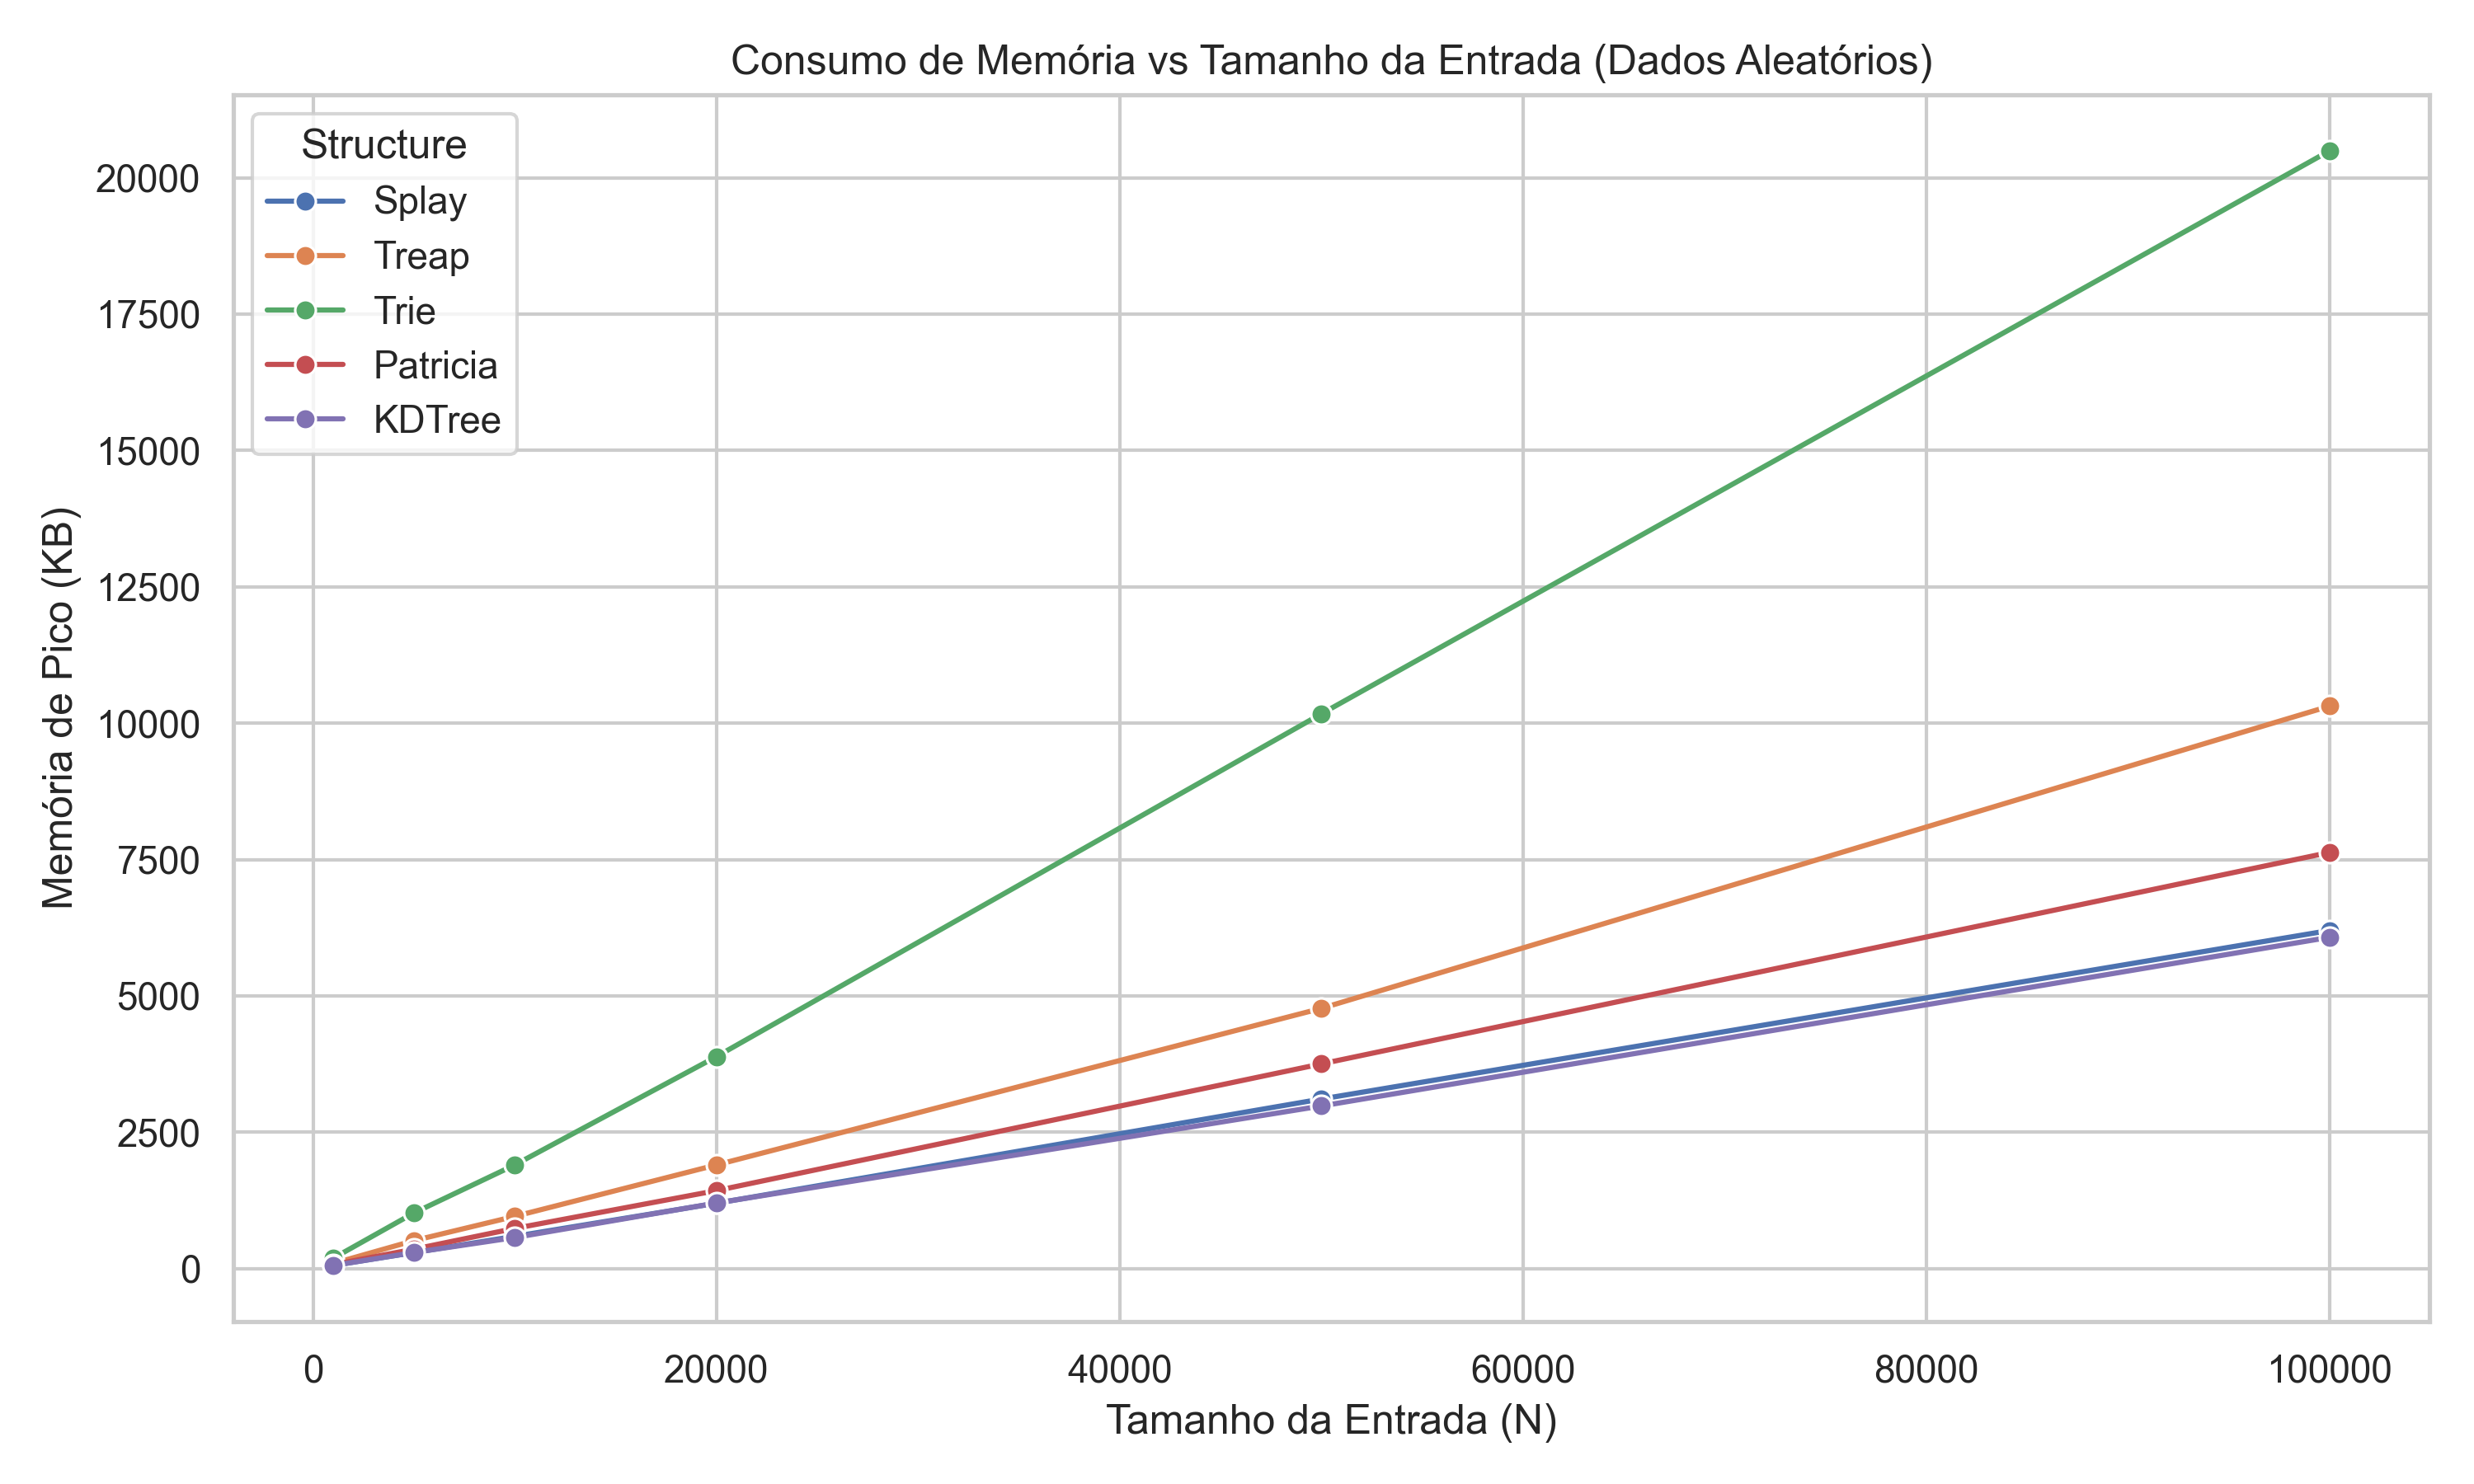
\includegraphics[width=0.75\textwidth]{memory_random.png}
    \caption{Peak Memory Consumption by the interpreter vs Number of Insertions.}
    \label{fig:memory}
\end{figure}

\subsection{Distributional Sensitivity (Worst Computational Case)}
Analyzing the structures with degenerate data (strictly ordered distribution along the array), the chart in Figure \ref{fig:worst} indicates the performance catastrophes of unadapted trees, notably visible if the KD-Tree receives inputs as uniform ordered pairs $(1,1), (2,2), ..., (n,n)$, reducing the multi-spatial topology to a mere oblique Linear Linked List $\mathcal{O}(N^2)$.

\begin{figure}[H]
    \centering
    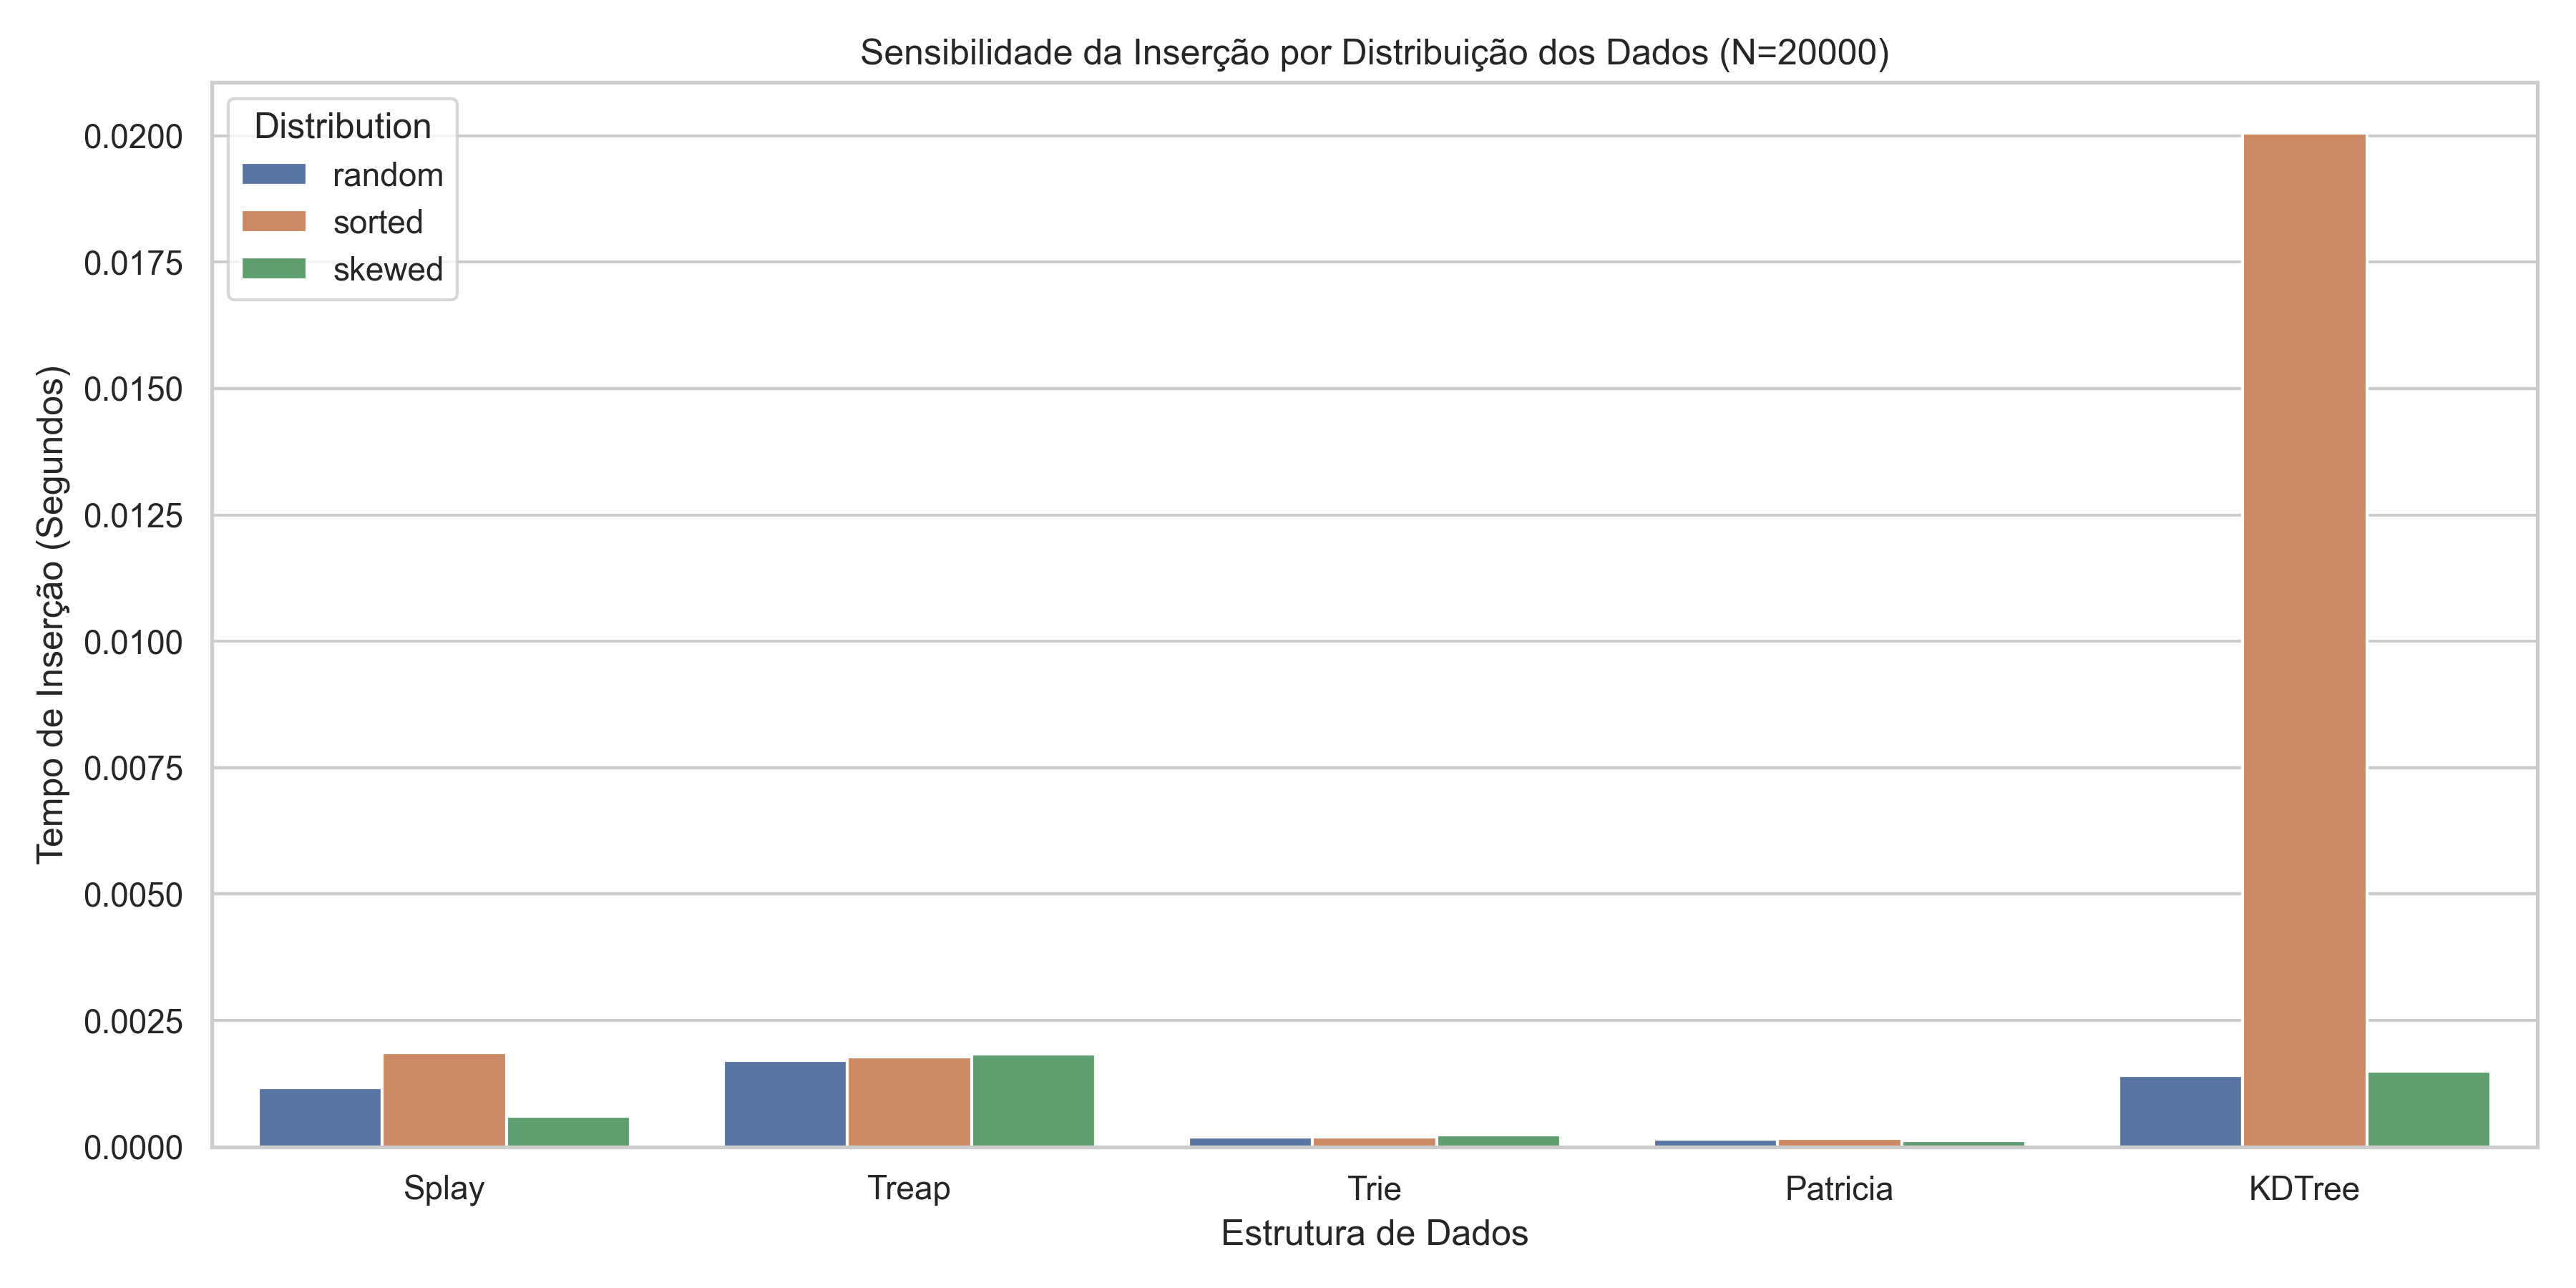
\includegraphics[width=0.75\textwidth]{distribution_impact.png}
    \caption{Impact of the worst computational case with static N.}
    \label{fig:worst}
\end{figure}

\section{Conclusion}
The experiment achieved the intended objectives in the AED 2 discipline. It was verified not only theoretically but visually and empirically that Advanced Tree Structures are ingenious products directed at the minutiae of systems architecture. While the Splay Tree revolutionizes the use of locality premises, the Patricia Tree shows how deep string handling can go to save RAM \textit{heaps} on modern servers. Finally, consolidating this into modern visual smartphone interfaces proves how timeless the fundamentals of computing theory truly are.

\end{document}
